%************************************************
\chapter{Michelson Interferometer}
%************************************************
\begin{flushright}
August 8 and 19, 2013 \\
% [$3 \times 6 hours spent$]
\end{flushright}

\section{Aim}
	To determine
	\begin{enumerate}
		\item the average wavelength of a monochromatic source 
		\item the difference in wavelengths of a dichromatic source (Sodium Light)
	\end{enumerate}
	and to obtain White Light fringes.

\section{Theory}
	The Michelson interferometer demonstrates interference by \emph{division of amplitude} of a wave by partial reflection. The apparatus consists of a source of light, two highly polished plane mirrors, a detector, a beam splitter and a compensating plate. The beam splitter is highly polished at the rear face in order to minimise reflections from the front face. The compensating plate made of the same material and adjusted parallel to beam splitter, essentially makes the path distance travelled in glass by both the beams equal, since one ray undergoes internal reflection while the other undergoes an external reflection; this is important in case the light is not monochromatic (for e.g white light) since refractive index changes with wavelength. \\
	\par
	When light from the source falls on the beam splitter, it is partially reflected and partially transmitted in orthogonal directions. These two beams reach the mirrors and are then reflected back into the detector. The fringes can be seen by looking into the mirror through the beam splitter. \\
	\par
	\autoref{e1} \footnote{Taken from Jenkins White} explains the formation of fringes. It can be understood by considering replacement of the real mirror $M_2$ by its virtual image ${M_2}'$ formed by reflection in $G_1$. ${M_2}'$ is parallel to $M_1$. We may now think of the source as forming two virtual images $L_1$ and $L_2$ in $M_1$ and ${M_2}'$. Looking at the mirror $M_1$, one can see $M_1$ along with the virtual image ${M_2}'$ of  $M_2$ formed in  $G_1$. The air film enclosed between $M_1$ and ${M_2}'$ is wedge shaped, and we obtain straight line fringes. Circular fringes are obtained when the interferometer is in normal adjustment. Depending on the shape of this air film i.e the angle between the mirrors the fringes can be straight, circular, parabolic, elliptical, hyperbolic in shape. \\
	\par
	In the given apparatus, both the mirrors can be moved with the help of screws and the distance moved can be measured with a precision of $10^{-7}m$. One of the mirrors is mounted on a carriage, whose movement mechanism consists of a large drum. One rotation of this drum moves the mirror by a millimetre.  One part of a slow motion smaller drum moves the mirror by $10^{-4}mm$. The beam splitter and compensating plate are aligned at $45^{o}$ to the interferometer arm. The mirrors are provided with two screws at the back which help tilt them so as to adjust them mutually perpendicular. \\
	\par
	\begin{figure}[bth]
		\begin{center}
			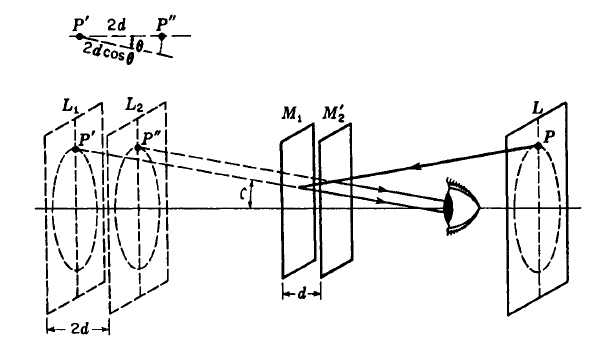
\includegraphics[width=1.1\linewidth]{gfx/e1}
		\end{center}
	\caption[Equivalent Michelson Interferometer Setup]{Equivalent Michelson Interferometer Setup}
	\label{e1}
	\end{figure}

	\subsection{Determining Wavelength}
		The easiest place to begin the analysis of this apparatus would be to ignore the thickness of the beam splitter and the compensator (which is anyway not needed for this experiment) and assume the observations are made at the centre of a far away screen (although in the experiment we've used a lens to focus at infinity). Now at this point, the path difference in the two beams of light would be essentially because of twice the distance between the fixed mirror and the image of the movable mirror. Let this be given by $2d$, where $d$ is the distance between the said mirrors. Now imagine a point other than than the centre at the screen. The angle this makes with the principal axis, let that be $\theta$. The distance light will travel for this point, which can cause phase difference will be $2d \cos{\theta}$. Keeping in mind the fact that there's an abrupt phase change of $\pi$ because of reflection at the beam splitter, we have for destructive interference
		\begin{equation}
			2d\cos{\theta}=m\lambda
		\end{equation}
		and similarly, for constructive interference we'll have
		\begin{equation}
			2d\cos{\theta}=(m+1/2)\lambda
		\end{equation}
		It is easy to put in a few numbers \footnote{refer to page 15.23 of Ajoy Ghatak, Optics, 4th Edition for details} and conclude that reducing the distance causes fringes to collapse to the centre (while the spacing between fringes increases).

		Now experimentally, say for a given configuration, the centre's dark;
		\begin{equation}
			2d=m\lambda
		\end{equation}
		where $2d$ again, represents the distance between the mirrors, but that is not known experimentally. What is known experimentally is the position of the moveable mirror, with respect to some reference, $d_i$.
		Now we move this mirror to a new position, say $d_f$, such that $N$ fringes have collapsed to the centre in the process. Then we have
		\begin{equation}
			2(d+ (d_f-d_i))=(m-N)/\lambda
		\end{equation}
		Subtracting these, gives us a simple method of finding the `average' wavelength of the sodium source
		\begin{equation}
			\lambda=2(d_f-d_i)/N=2\Delta D/N
			\label{5_eq1}
		\end{equation}


	\subsection{Resolving the D-Lines}
		That was the basic theory behind the experiment. Using a little more naive Math, we can even find the small difference in the Sodium D-lines. Here's how we go about it. As a though experiment, imagine that `$d$' is made 0. Then the mirror is moved away (or towards) through a distance $d$. In general, the fringe patterns will overlap in some fashion. Assume a $d$ is such that,
		\begin{equation}
			2d\cos{\theta}=m\lambda_1 \\
			2d\cos{\theta}=(m+1/2)\lambda_2
		\end{equation}
		For small $\theta$, we can easily obtain
		\begin{equation}
			2d/\lambda_1 - 2d/\lambda_2 = 1/2
		\end{equation}
		Observe here what has happened. The maxima of one pattern falls on the minima of the other and vice versa. This means that what we obtain is all bright! Consequently, the pattern disappears in this situation. Making this general, if
		\begin{equation}
			2d/\lambda_1 - 2d/\lambda_2 = 1/2, 3/2, 5/2 ..
		\end{equation}
		then the fringe pattern will disappear and for 1, 2, 3 .. it will reappear. 
		Now let us think about how this could be achieved in practice, as it is hard to find the precise location where $d$ becomes zero. To get around this, we find the distance between occurrence of two blank (all bright) patterns. Assuming the unknown (to the experimenter) distance between the mirrors is $d$, but the position of the moveable mirror with respect to some reference, is again given by $d_i$. We can then write in general for some odd $m$
		\begin{equation}
			2d (1/\lambda_1 - 1/\lambda_2) = m/2
		\end{equation}
		Now the moveable mirror is moved to a position $d_f$ such that the same pattern is obtained. For this we then have
		\begin{equation}
			2(d+(d_f-d_i)) (1/\lambda_1 - 1/\lambda_2) = m/2 - 1
		\end{equation}
		On subtracting, to eliminate the unknown $d$, we get
		\begin{equation}
			2\Delta d (\Delta \lambda / \lambda^2) = 1
		\end{equation}
		where $\Delta d = d_f - d_i$. So finally we have,
		\begin{equation}
			\Delta \lambda = \lambda^2/2\Delta d
		\end{equation}
		and that's that.

	\subsection{Subtle Points}
		The theory discussed above is roughly sufficient. Finer points have been posed as questions % and then discuss them to develop a better understanding of the subject.
		\begin{enumerate}
			\item How does the diffuser help? Can the interference pattern be obtained without the diffuser?		
			\item What is the wavefront of the waves after they go through a diffuser?
			\item Why are the fringes circular? Explain using Huygen's principle (the ray optic method is rather simple).
			\item Are the fringes real or virtual?
			\item If the light source was in fact a point source, what type of an interference pattern will you obtain? (courtesy sir)
			\item In a typical YDSE setup, if we don't use a screen, are we expected to observe fringes?
			\item How can we span all angles using just two knobs in the mirror?
			\item Can you apply the idea of beats to explain the increase decrease of contrast?
			\item What is the expected pattern for a plain wavefront?
			\item For a plain wavefront, when a `dark' pattern is obtained (you'll know once you solve the previous question), where does the energy of the electromagnetic wave disappear? (sir asked this)
		\end{enumerate}
	
	\subsection{`Practical' Theory}
		Some more questions whose answers become clear after playing with the apparatus for sufficiently long
		\begin{enumerate}
			\item What is the primary source of the backlash error in the fine rotation knob?
			\item When the average distance of the mirrors from the partly reflecting mirror is higher, why is it harder to get circular fringes?
			\item What can cause a uniform rotation of the knob to screw (threaded cylinder) to not cause a corresponding change in the fringe pattern? (basically identify the main cause of this error)
		\end{enumerate}

\section{Procedure}	
	\subsection{Obtaining the ring}
		It is assumed that you've setup the michelson interferometer in accordance with the diagram in Jenkins White.
		\begin{enumerate}
			\item Move the coarsely moveable mirror to (roughly) the smallest distance from the beam splitter.
			%\item Move the coarsely moveable mirror to roughly an equal distance from the beam splitter as the other mirror
			%	using the pin hole disk, observe the image of the pinhole in the mirror. you will see two sets of images one for each mirror. using the screws provided at the back of the 
			\item Now move the other mirror to a slightly larger (you can use smaller also, but then the steps would change correspondingly) distance from the beam splitter, than that of the coarsely movable mirror.
			\item Ensure that the pin hole disk is being used.
			\item Align the mirror using the three screws provided such that all the four spots coincide (you can choose to look directly without the telescope; in fact that works better usually).
			\item Now remove the pin hole disk from the view and put the diffuser (if not already present).
			\item Move the moveable mirror at most four times using the coarse movement drum (ensure the movement knob is unlocked) until the fringe pattern is observed. If the pattern is too dense (more than roughly 15 fringes), then follow from the mirror alignment step.
			\item Assuming you have roughly 10 fringes at this stage, you now need to bring the centre of the rings into view (if it is already, you're running on beginner's luck).
			\begin{enumerate}
				\item There are two screws on the mirror and they can roughly be thought of as adjusting the X and Y offset.
				\item You'll know you're on the right track if the fringes magnify as you adjust
				\item Note that you must leave the knob to know where it really is. Simply holding it also causes the position of the knob to change.
			\end{enumerate}
			\item If you want further magnification, you can continue rotating and aligning the centre as you go if the need be.
		\end{enumerate}
		CAVEAT: For certain path differences, the contrast will become very low (as is clear from theory); don't panic.
	\subsection{Finding $\lambda_\text{average}$}
		Assuming you have obtained the ring already;
		\begin{enumerate}
			\item Set the movement to fine using the lock knob on the apparatus.
			\item Place the telescope if you haven't done that already, such that one of the rings is just at the cross-wire.
			\item Move the fine rotation knob until the fringes just start to move.
			\item Now keep track of the rotations and count 20 fringes as they cross the cross-wire.
			\item Repeat this to get sufficient observations			
		\end{enumerate}
	\subsection{Finding $\lambda_\text{separation}$}
		Assuming you've obtained the ring;
		\begin{enumerate}
			\item Lock the movement to fine using the lock knob
			\item Move the fine rotation until all the fringes disappear and just begin to appear
			\item Note the position at this point
			\item Now continue rotating the knob until the fringes disappear again and just begin to appear
			\item Note this position again
			\item Repeat this to get sufficient observations
		\end{enumerate}

\section{Observations and Conclusion}
	In accordance with \autoref{1_observations}, the wavelength of sodium light (average) was found to be $620 \pm 65nm$. \autoref{1_observations2}, the difference in wavelengths was found to be $0.67 \pm 0.15 nm$.
	\begin{figure}[bth]
		\begin{center}
			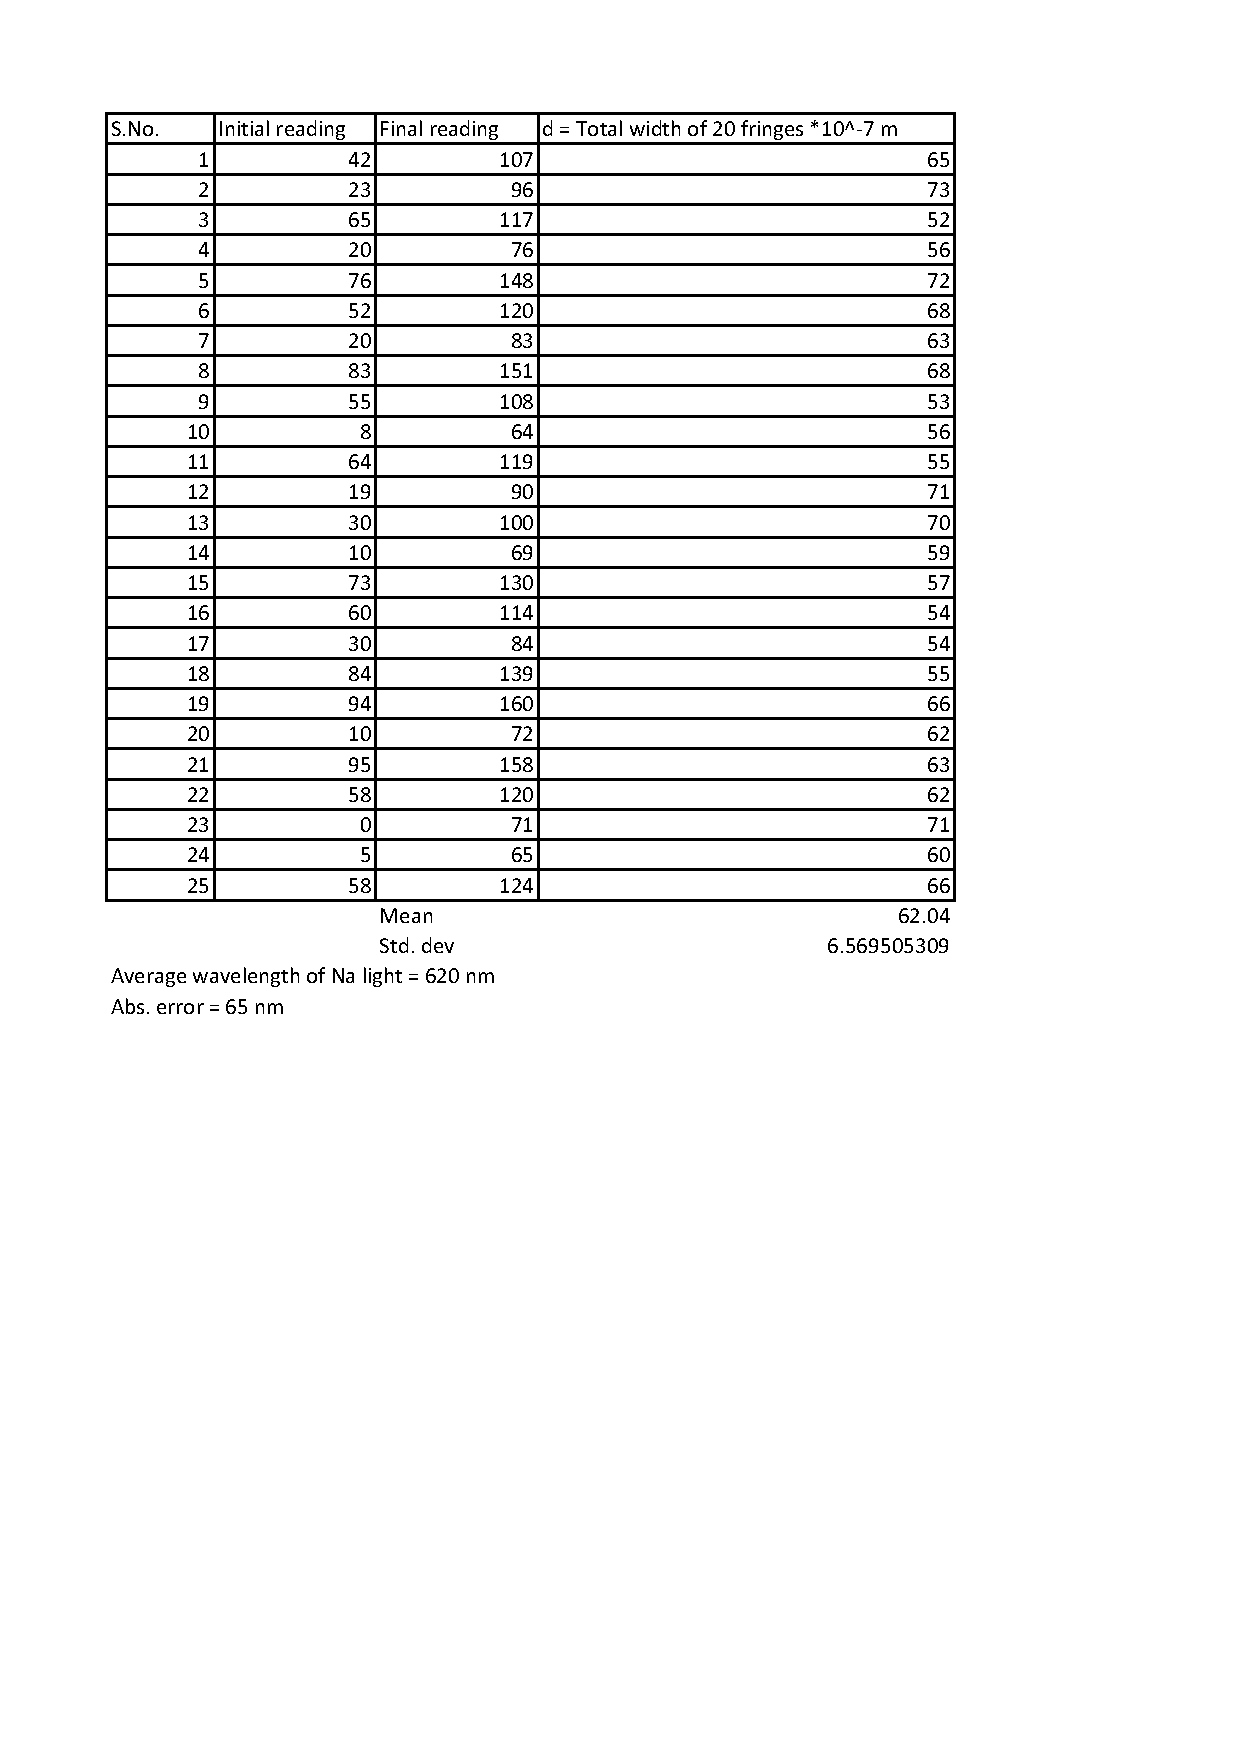
\includegraphics[width=1.3\linewidth]{gfx/1_obsA}
		\end{center}
		\caption[Observations for $\lambda_\text{average}0$]{Michelson Interferometer: Observations}
	\label{1_observations}
	\end{figure}
	\begin{figure}[bth]
		\begin{center}
			
\includegraphics[width=1.3\linewidth]{gfx/1_obsB}
		\end{center}
		\caption[Observations for $\lambda_\text{difference}0$]{Michelson Interferometer: Observations}
	\label{1_observations2}
	\end{figure}


\section{Sources of error}
	\begin{itemize}
		\item The back and  forth movement of the mirrors is not precise i.e. the mirrors do not remain parallel to the preceding positions. So the setup might not be normally adjusted and the fringes might not be circular.
		\item The large drum has a gear arrangement that is aligned to move with the thread of the screw. This calls for a significant amount of backlash error which means that while the screw moves, the fringes don't contributing to erroneous results.
		\item While noting the positions when the fringes reappear, the contrast of the fringes is noted by the human eye. This contrast almost doesnot vary over almost a rotation of the small screw. 
	\end{itemize}

